В наши дни, когда компьютерные технологии бурно развиваются, не
всегда удается создать сложное приложение, используя один язык
программирования. Разные языки имеют свои преимущества и недостатки и как
правило, что ни один из них не удовлетворят требованиям разрабатываемой
прикладной программы. Выходом из такого положения является использование
нескольких языков программирования. Такой подход часто используется при
создании программ для научных исследований, управления производственными
процессами и других коммерческих приложений. При этом приходится решать
задачи взаимодействия компонентов, написанных, которые написаны на на
разных языках программирования. Компоненты, реализующие графический
интерфейс пользователя, управление базами данных, получение и обработку
данных в реальном времени, как правило интегрируются в одно приложение.

Для реализации поставленной задачи исследования в магистерской
диссертации был выбран пакет моделирования процессов столкновения элементарных частиц при высоких энергиях на ускорителях элементарных частиц \textit{PYTHIA} на языке программирования \textit{С++}, а также принято решение о реализации всего программного
комплекса на языке программирования \textit{Java}.
В качестве веб интерфейса был использован фреймворк \textit{Angular} на языке программирования \textit{JavaScript}. Так же была использована и бибилотека \textit{d3js} для отрисовки графиков в виде \textit{SVG} изображений и взаимодейсвия пользователся с интерфейсом приложения.

Когда говорят о научных основах проектирования пользовательских
интерфейсов, в первую очередь упоминают термин \textit{Human-Computer Interaction}
(\textit{HCI}) – «взаимодействие человека и компьютера». В странах Запада \textit{HCI} это
является целой профессией, ей обучают в университетах, издается много
журналов по этой теме, существует большое количество Web-сайтов.
Составными частями \textit{HCI} являются:

\begin{enumerate}
	\item[--] человек (пользователь);
	\item[--] компьютер;
	\item[--] их взаимодействие.
\end{enumerate}

Пользовательский интерфейс \textit{user interface} (\textit{UI}) – является своеобразным
коммуникационным каналом, по которому осуществляется взаимодействие
пользователя и компьютера.

Лучший пользовательский интерфейс – это такой интерфейс, которому
пользователь не должен уделять много внимания, почти не замечать его. В руках
пользователя интерфейс пользователя должен служить инструментом для
достижения цели. Такой интерфейс называют прозрачным – пользователь
смотрит сквозь него на свою работу.

Чтобы создать эффективный интерфейс, который делал бы работу с
программным комплексом эффективной, нужно понимать, какие задачи будут
решать пользователи с помощью данной программного комплекса и какие
требования к интерфейсу могут возникнуть у пользователей. Большую роль в
разработке интерфейса играет интуиция – если разработчик сам терпеть не
может некрасивые и неудобные интерфейсы, то при создании собственного
программного комплекса он будет чувствовать, где и какой именно элемент
нужно убрать или добавить. Необходимо иметь художественный вкус, чтобы
понимать, что именно придаст интерфейсу красоту и привлекательность.

Западные исследователи в области \textit{HCI} сформулировали основные
принципы проектирования пользовательских интерфейсов компьютерных
программ~\cite{user-interface}. Как и в любой другой отрасли ИТ, существует довольно много
различных методик и классификаций. Можно сформировать три положения
говоря об общих принципах проектирования пользовательского интерфейса:

\begin{enumerate}
	\item[--] программный комплекс должен помогать выполнить задачу, а не
	становиться этой задачей;
	\item[--] при работе с программой пользователь не должен думать, что он не
	понимает программу;

	\item[--] программный комплекс должен работать так, чтобы пользователь не
	считал компьютер бесполезным инструментом.
\end{enumerate}

Конечно, глубина проработки интерфейса и степень его адаптивности под
нужды пользователя в программных комплексах в основном зависит от усилий
их авторов, а не от характеристик аппаратного обеспечения. Однако у
большинства пользователей компьютер ассоциируется именно с программными
комплексами, которые на нем работают, и плохое впечатление от использования
программного обеспечения автоматически переносится на сам компьютер.

Сообщество разработчиков фреймворка \textit{Angular} разрабатывает дополнительные компоненты \textit{Angular Material Design} и предлагает использовать их для быстой разработки приложения с нуля. 

\textit{Material Design} -- визуальный язык, представлен в 2014 году \textit{Google}, используется чаще всего в мобильных приложения. Пример использования \textit{Material Design} можно увидеть во многих мобильных приложения Google(Play, Music, Books и т.д.), а также в Chrome OS. Material Design упрощает разработчикам настройку UI, сохраняя при этом удобный интерфейс приложений. Angular Material состоит из набора предустановленных компонентов Angular. Anglate Material стремится обеспечить расширенный и последовательный пользовательский интерфейс. В то же время он дает возможность контролировать, как ведут себя разные компоненты.

Открыв начальную веб-страницу приложения в любом из доступных браузеров пользователь увидит сообщение с описанием проекта, как показано на рисунке~\ref{fig:welcome-page}.

\vspace{16pt}
\begin{figure}[!h]
	\centering
	
\includegraphics[width=\textwidth]{figures/welcome-page.png}
	\caption{Начальная \textit{web}-страница}
	\label{fig:welcome-page}
\end{figure}

Для каждого пользователя на начально странице приложения распологается навигационное меню, котрое показано на рисунке~\ref{fig:menu}. Так как разработанное приложение является одностраничным то переход по пунктам меню не перезагружает страницу полностью, а лишь догружает необходимые компоненты.

\begin{figure}[!h]
	\centering
	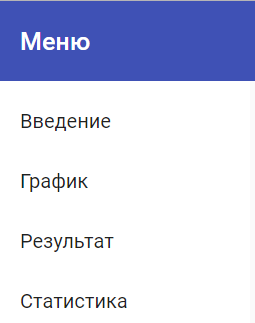
\includegraphics[width=0.5\textwidth]{figures/menu.png}
	\caption{Навигационное меню приложения}
	\label{fig:menu}
\end{figure}
\vspace{5cm}
Из главного меню доступен переход на следующие страницы приложения: 

\begin{enumerate}
	\item[--] <<Введение>> -- начальная страница \textit{web}-приложения;
	\item[--] <<График>> -- страницы с основным графиком и панелью для ввода параметров и отравки запроса на вычисление;
	\item[--] <<Результат>> -- страница предосталяющая полученные результаты на угол смешивания ${Z}^{\prime}$-бозонов в модели \textit{SSM};
	\item[--] <<Статистика>> -- страница со статистикой приложения;
\end{enumerate}

Перейдя на страницу <<График>> пользователь увидет пустой график распределения теоретического сечения кросс-секции $\sigma \times Br({Z}^{\prime} \rightarrow {W}^{+}{W}^{-})$ для ${Z}^{\prime}_{SSM}$ и множество панелей управления, которые позволяют отправить запрос на начало эмуляции процесса $pp \rightarrow {W}^{+}{W}^{-} + X$ в протон-протонном столкновении. 

Для начала старта генерации собыйтий необходимо заполнить значение кси ($\xi$), количество моделируемых событий и количество циклов моделирования одного значения на графике для одного значения массы ${M}_{{Z}^{\prime}}$. Данная панель показана на рисуноке~\ref{fig:request-line}
% ... с началом массы ${M}_{{Z}^{\prime}}$ и шагом


\vspace{16pt}
\begin{figure}[!h]
	\centering
	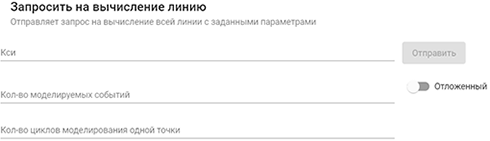
\includegraphics[width=\textwidth]{figures/request-line.png}
	\caption{Панель старта расчета линии значений}
	\label{fig:request-line}
\end{figure}

После выставления нужных пользователю параметров, необходимо нажать кнопку <<Отправить>> после чего данные отправяться на сервер и результат будет перерисован на интерфейсе приложения. Результаты вычислений будут добавлены на основной график в реальном времене, поэтому пользователю не нужно обновлять страницу с графиком.

Как только запрос был отправлен на сервер соездается \textit{websocket} соединение между \textit{web}-браузером пользователя и серверным приложением, тем самым подписывая клинта на получени денных от сервера, как только они будут готовы.

На графике кросс-секции $\sigma \times Br({Z}^{\prime} \rightarrow {W}^{+}{W}^{-})$ для ${Z}^{\prime}_{SSM}$ отриросовывается линия с новыми значениями в то время, как серверное приложение начинает параллельно для нескольких значений массы ${M}_{{Z}^{\prime}}$ моделировать столкновение протонов.

Так как в реальном столкновении протонов рождается очень большое количество различных частиц то моделирование такой задачи при помощи генератора \textit{PYTHIA} требудет значительных ресурсов центрального процессора сервера и занимает продолжительное время. Приложение созданное в рамках данной работы имеет \textit{web}-интерфейс, что позволяет сразу нескольком пользователям работать в нем и отправлять запросы на вычичления. В связи с этим вводится ограничение на количество параллельно зарпущеных процессов моделирования для каждого пользователя.

Даже самая простая задача расчета модели занимает большое время. К примеру запрос пользователя расчитать линию для всех значений ${M}_{{Z}^{\prime}}$, а в рамках данного проекта это пять тысячь точек на графике от 0 до 5000 ГэВ, и количеством генерируемых собыйтий займет 9,7 часа. 

В таком простом случае полученное значение будет подвержено значительной статистической ошибки. Чтобы убрать данную статистическую ошибку тербуются дополнительные циклы имметационного моделирования, что увеличивает затраченное время в разы. 

Под панелью для запроса вычислений распологается список ранее отправильных запросов, как показано на рисунке~\ref{fig:preferences}. Нажав на крестик <<X>> можно удалить линию на графике.

Все запросы на вычисление сохраняются для конкретного пользователя и загружаются из локального хранилища данных при обновлении страницы.

\begin{figure}[!h]
	\centering
	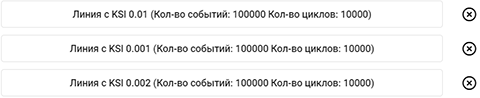
\includegraphics[width=\textwidth]{figures/preferences.png}
	\caption{Список отображаемых линий}
	\label{fig:preferences}
\end{figure}

Так как вычисления могут занять довольно много времени
Для удобства вычисления линий была добавлена возможно отправить запрос на отложенные вычисления 

Предусмотрена возможность отправлять запросы на вычисление только одной точки... .

\begin{figure}[!h]
	\centering
	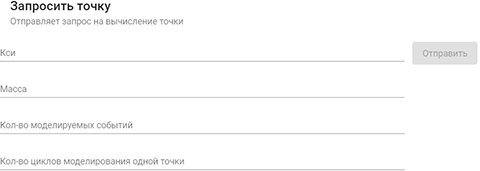
\includegraphics[width=\textwidth]{figures/request-point.png}
	\caption{Панель старта расчета одного значения}
	\label{fig:request-point}
\end{figure}

Процесс вычиления всех значений для ${M}_{{Z}^{\prime}}$

\begin{figure}[!h]
	\centering
	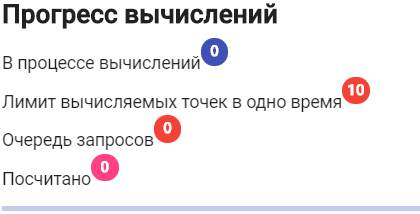
\includegraphics[width=\textwidth]{figures/progress.png}
	\caption{Панель старта расчета линии значений}
	\label{fig:progress}
\end{figure}

Интерфейс результатов и вычислений состоит из

\begin{figure}[!h]
	\centering
	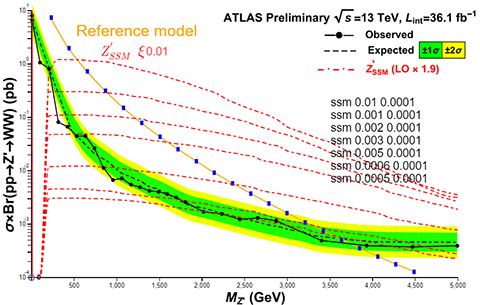
\includegraphics[width=\textwidth]{figures/graph-1.png}
	\caption{Панель старта расчета линии значений}
	\label{fig:graph-1}
\end{figure}

\begin{figure}[!h]
	\centering
	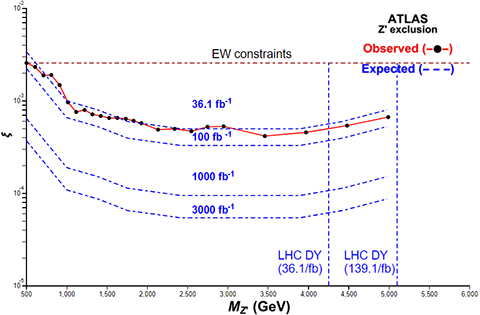
\includegraphics[width=\textwidth]{figures/graph-result.png}
	\caption{Панель старта расчета линии значений}
	\label{fig:graph-result}
\end{figure}

Так же реализована возможность смены языка на котором отображается текст приложения в правом верхне углу \textit{web}-интерфейса


